\subsection{Результаты моделирования}
На основе библиотеки SkyNet~\cite{lippuner2017} мы подготовили программу, симулирующую $r$-процесс в выбросе вещества при слиянии двух нейтронных звезд. Термодинамические параметры были заданы так, как описано в разделе~\ref{sec:nsm}. Мы провели три симуляции, использующие разные библиотеки астрофизических реакций, составленные нами с использованием трех таблиц теоретических масс ядер: FRDM2012~\cite{moller2016}, HFB-24~\cite{goriely2013} и LMR2021~\cite{vladimirova2022}. В этом подразделе представлены результаты наших расчетов и анализ чувствительности модели $r$-процесса к массам задействованных изотопов.

\subsubsection{Итоговые выходы $r$-изотопов}

\begin{figure}
\centering
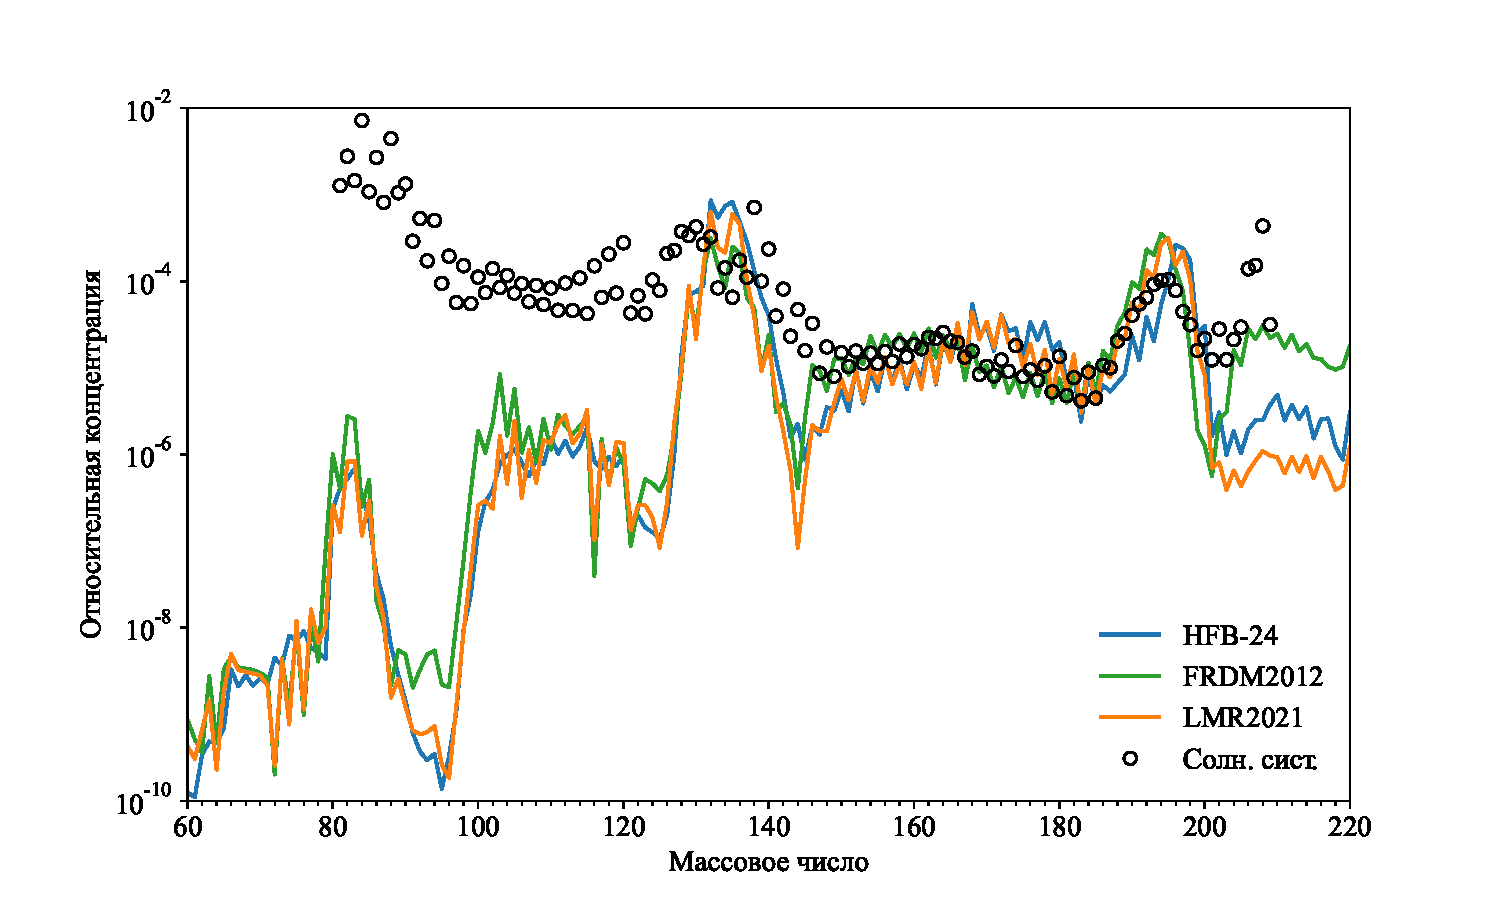
\includegraphics[width=0.9\textwidth]{pics/distr.pdf}
\caption{Массовые распределения продуктов $r$-процесса, полученные в симуляциях нуклеосинтеза длительностью 1 секунда с разными массовыми моделями, и наблюдаемые в Солнечной системе распространенности ядер с $A \geq 80$~\cite{lodders2003}. Экспериментальные данные нормированы по участку $145 \leq A \leq 185$ теоретических распределений.}
\label{fig:distr}
\end{figure}

На рис.~\ref{fig:distr} представлены выходы продуктов $r$-процесса через 1 секунду симуляции. На полученные нами массовые распределения наложены данные о наблюдаемых в Солнечной системе распространенностях изотопов с $A \geq 80$. Отметим, что мы моделировали изолированный односекундный $r$-процесс в сценарии слияния нейтронных звезд, в то время как экспериментальное распределение складывалось на астрофизических масштабах времени в результате множества механизмов нуклеосинтеза, поэтому сравнивать их мы будем лишь на качественном уровне. В частности, как и в прочих работах (например,~\cite{goriely2011}), полученное массовое распределение расходится с экспериментальными на многие порядки, так как в этой области основной вклад должны вносить $s$-процесс и слабый $r$-процесс.

Использованная нами модель нуклеосинтеза воспроизводит основные свойства наблюдаемых распространенностей тяжелых ядер: хорошо видны три пика $r$-процесса с $A \approx 80 - 88$, $128 - 142$, $190 - 200$, соответствующие магическим числам нейтронов. Как говорилось выше, экспериментальные пики $r$-процесса смещены относительно пиков $s$-процесса, так как ядра, рождающиеся при быстром захвате нейтронов, далеки от долины стабильности и быстро распадаются. Мы симулируем односекундный $r$-процесс, поэтому полученные нами пики с $A \approx 128 - 142$ находятся между экспериментальными пиками $r$- и $s$-процесса, находясь в процессе размытия вследствие распадов. В области тяжелых ядер размытие происходит значительно быстрее, поэтому полученные нами максимумы с $A \approx 190 - 220$ совпадают с экспериментальным третьим пиком $r$-процесса.

Рис.~\ref{fig:distr} позволяет оценить чувствительность симуляции $r$-процесса к теоретическим ядерным массам. Видно, что вариация массовой модели приводит к значительным расхождениям распределений $r$-изотопов. Выходы в симуляции с массовой таблицей FRDM2012 почти везде превышают выходы остальных симуляций, для некоторых значений $A$ на многие порядки. Это хорошо заметно для ядер с $A \geq 200$. При этом в области $164 \lesssim A \lesssim 182$, где массовое распределение FRDM2012, наоборот, ниже остальных распределений, оно повторяет профиль экспериментальных данных.

\begin{figure}
  \centering
  \begin{subfigure}{0.32\textwidth}
    \centering
    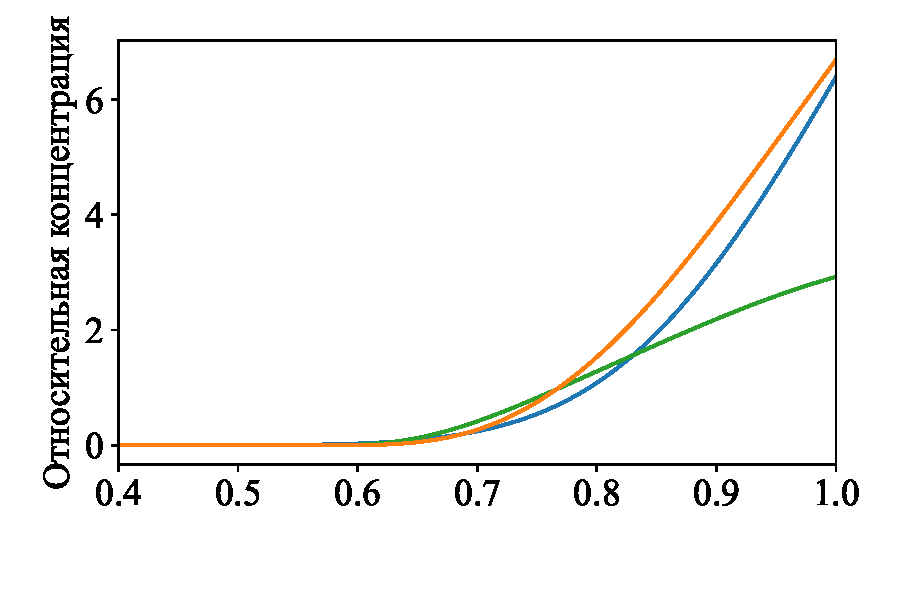
\includegraphics[width=\textwidth]{pics/y_65_176.pdf}
    \caption{${}^{176}$Tb}
  \end{subfigure}
  \hfill
  \begin{subfigure}{0.32\textwidth}
    \centering
    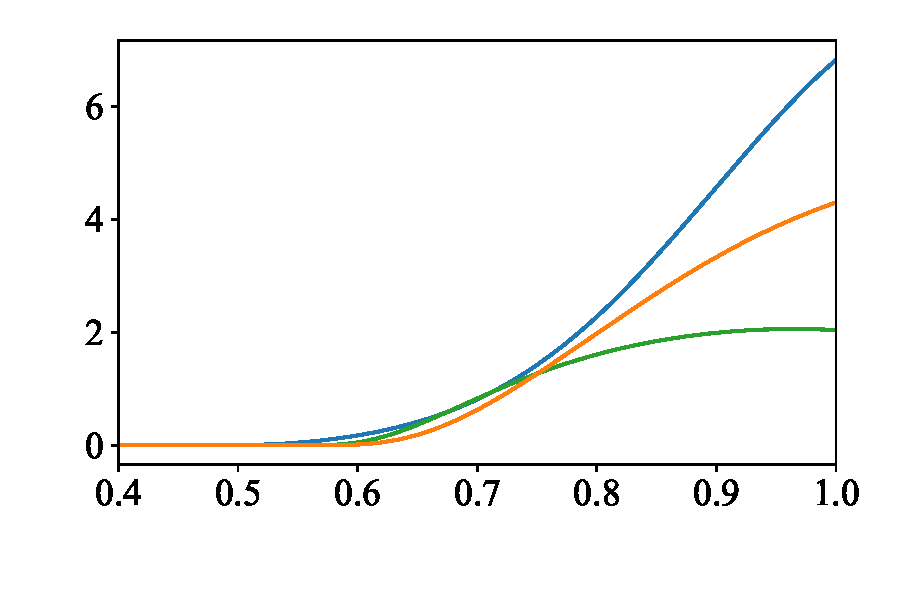
\includegraphics[width=\textwidth]{pics/y_65_178.pdf}
    \caption{${}^{178}$Tb}
  \end{subfigure}
  \hfill
  \begin{subfigure}{0.32\textwidth}
    \centering
    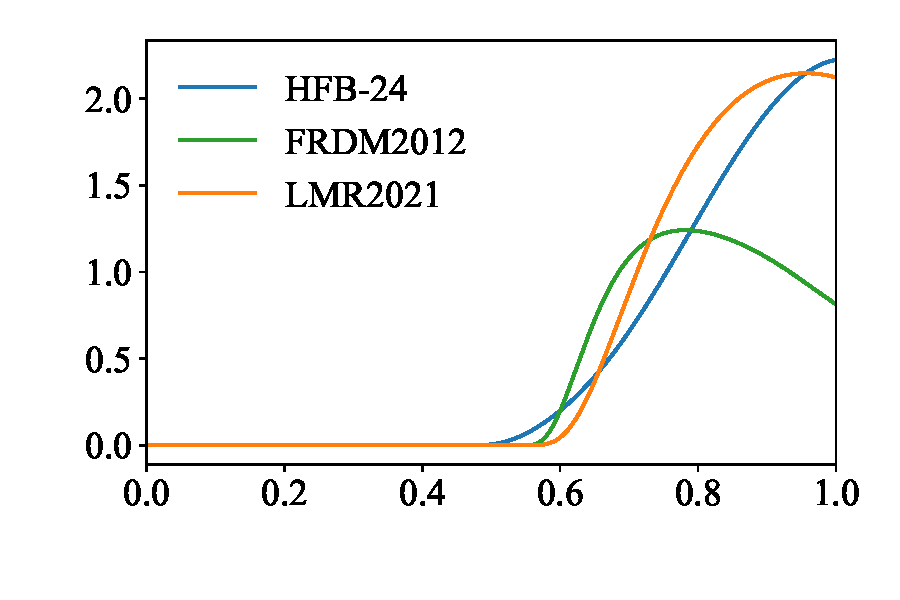
\includegraphics[width=\textwidth]{pics/y_65_180.pdf}
    \caption{${}^{180}$Tb}
  \end{subfigure}
  
  \vspace{0.3cm}
  \begin{subfigure}{0.32\textwidth}
    \centering
    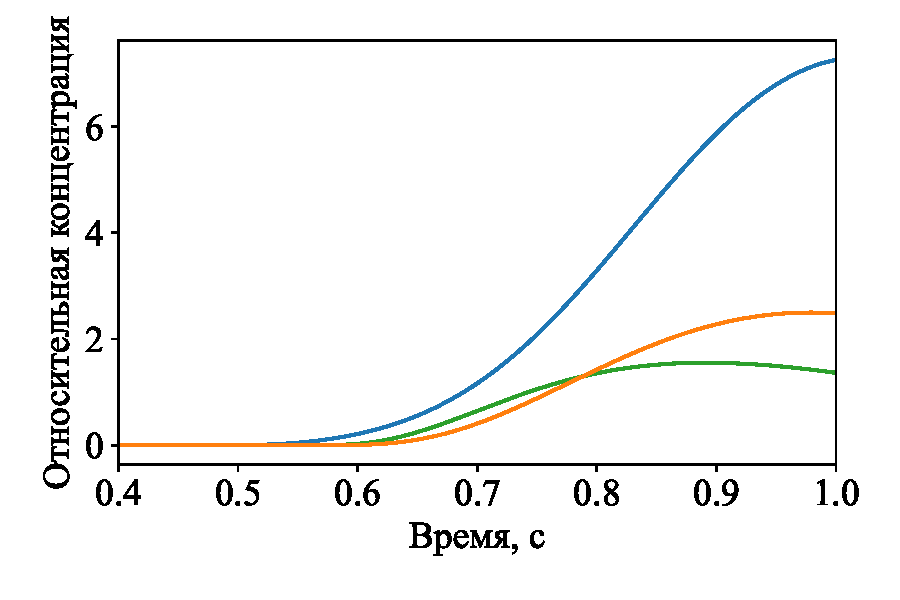
\includegraphics[width=\textwidth]{pics/y_65_177.pdf}
    \caption{${}^{177}$Tb}
  \end{subfigure}
  \hfill
  \begin{subfigure}{0.32\textwidth}
    \centering
    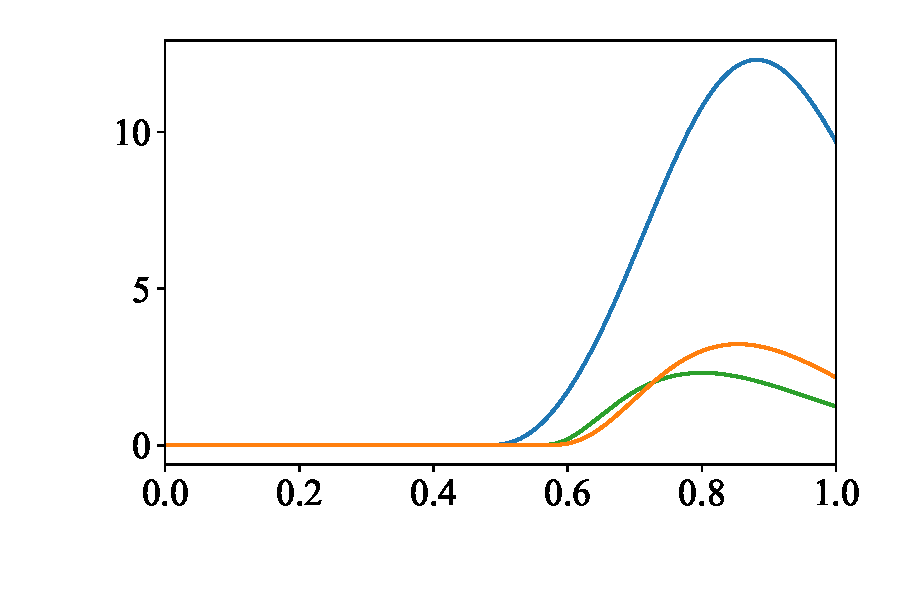
\includegraphics[width=\textwidth]{pics/y_65_179.pdf}
    \caption{${}^{179}$Tb}
  \end{subfigure}
  \hfill
  \begin{subfigure}{0.32\textwidth}
    \centering
    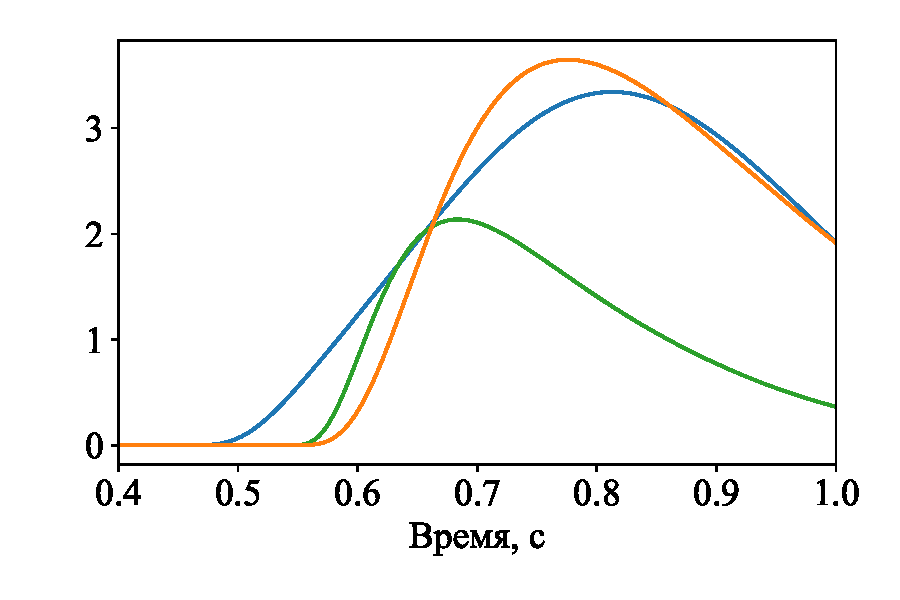
\includegraphics[width=\textwidth]{pics/y_65_181.pdf}
    \caption{${}^{181}$Tb}
  \end{subfigure}
  \caption{Эволюция концентраций нейтроноизбыточных изотопов тербия в симуляциях $r$-процесса с использованием различных массовых моделей. В верхнем ряду представлены четно-нечетные ядра, в нижнем --- нечетно-нечетные. Теоретические концентрации отнормированы, как на рис.~\ref{fig:distr}, и домножены на $10^6$.}
  \label{fig:tb-evolution}
\end{figure}

Массовые распределения FRDM2012 и LMR2021 для некоторых массовых чисел демонстрируют схожие глубокие провалы, например, на промежутке $A = 73 - 78$. Такие поведение может быть вызвано микроскопическими ядерными эффектами, так как эти минимумы коррелируют с изменением четности $A$. Также FRDM2012 и LMR2021 предсказывают схожие зубчатые формы максимума в области $A = 100 - 106$. HFB-24 эти особенности не воспроизводит или воспроизводит не так заметно, предсказывая там более гладкое поведение массового распределения. По-видимому, FRDM2012 и LMR2021 в одинаковой степени чувствительны к четности ядер. Заметим, что в методе LMR2021 микроскопические эффекты явным образом не учитываются.

\subsubsection{Эволюция выходов $r$-изотопов}

\begin{figure}
  \foreach \n in {200, 500, 800}{
    \centering
    \begin{subfigure}{\textwidth}
      \centering
      \begin{subfigure}{0.32\textwidth}
        \centering
        \includegraphics[width=\textwidth]{pics/evo_frdm2012_\n}
      \end{subfigure}
      \hfill
      \begin{subfigure}{0.32\textwidth}
        \centering
        \includegraphics[width=\textwidth]{pics/evo_hfb24_\n}
      \end{subfigure}
      \hfill
      \begin{subfigure}{0.32\textwidth}
        \centering
        \includegraphics[width=\textwidth]{pics/evo_lmr2021_\n}
      \end{subfigure}
      \caption{$t = \n$~мс}
    \end{subfigure}
    
    \vspace{0.3cm}
  }
  \caption{Выходы $r$-изотопов в симуляциях с разными массовыми моделями: в левом столбце FRDM2012, по центру HFB-24, в правом столбце LMR2021. Нормировка концентраций такая же, как на рис.~\ref{fig:distr}. Пустыми квадратами отмечены стабильные изотопы.}
  \label{fig:evolution}
\end{figure}

Более детально изучить влияние массовой модели на симуляцию $r$-процесса можно по изменению концентраций изотопов во времени. На рис.~\ref{fig:tb-evolution} представлены графики выходов нейтроноизбыточных изотопов тербия в $r$-процессе. Заметный синтез этих ядер в $r$-процессе начинается по прошествии $0.5 - 0.6$ секунд с начала симуляции, однако это время зависит от выбора массовой модели. Это можно объяснить изменением порогов реакций, в которых рождаются эти изотопы. По графикам выходов ${}^{177}\text{Tb}$, ${}^{178}\text{Tb}$ и ${}^{179}\text{Tb}$ хорошо видно, что вариация массовой модели может приводить к изменениям концентраций изотопов в разы. Как видно по рис.~\ref{fig:distr}, эти различия могут складываться в расхождения на порядки между итоговыми массовыми распределениями. Для некоторых изотопов видны максимумы зависимостей концентрации от времени. Образовавшись в каком-то количестве, они начинают распадаться и фотодиссоциировать при нарушении статистического баланса. Положение этих максимумов также зависит от выбора массовой модели.

На рис.~\ref{fig:evolution} зафиксированы выходы изотопов в диапазоне $N = 40 - 160$ и $Z = 30 - 90$ по прошествии 200, 500 и 800 мс с момента начала симуляции. Видно, что $r$-процесс очень быстро доходит практически до линий отделения нейтронов, формируя на $NZ$-диаграмме узкую полоску с преобладающими выходами изотопов. Форма и устойчивость пути $r$-процесса обеспечиваются за счет статистического баланса между реакциями $(n,\gamma)$ и $(\gamma,n)$, а также $\beta$-распадами, за счет которых становится возможным рождение новых химических элементов. С течением времени и изменением термодинамических условий, влияющих на статистический баланс, путь $r$-процесса расползается и отходит от границы существования ядер ближе к долине стабильности, отмеченной на рис.~\ref{fig:evolution} пустыми квадратами. При этом время, которое система находилась в состоянии статистического баланса, различается в трех расчетах: видно, что к середине симуляции (рис.~\ref{fig:evolution}, средний ряд) в расчетах с таблицами масс FRDM2012 и LMR2021 путь $r$-процесса все еще узок и прижат к линии отделения нейтронов, а в расчета с HFB-24 статистический баланс между реакциями нейтронного захвата и фотодиссоциации сместился ближе к долине стабильности. Таким образом выбор модели для расчета масс нейтроноизбыточных ядер влияет не только на выходы $r$-изотопов, но и на длительность течения и интенсивность $r$-процесса.

\subsubsection{Эволюция термодинамических параметров}
От выбора астрофизического сценария зависят важнейшие термодинамические величины влияющие на протекание $r$-процесса. В то же время многие процессы в астрофизике напрямую обусловлены ядерными реакциями. Любопытно пронаблюдать, как выбор модели масс ядер может повлиять на макроскопические параметры модельной системы.

Как говорилось выше, в нашей симуляции нуклеосинтеза учитывается энерговыделение реакций, что должно приводить к дополнительному нагреву остывающего вещества, выброшенного при столкновении нейтронных звезд. Чувствительность термодинамических параметров к вариации масс нейтроноизбыточных ядер можно пронаблюдать по зависимости температуры системы от времени, представленной на рис.~\ref{fig:temp}.

\begin{figure}
\centering
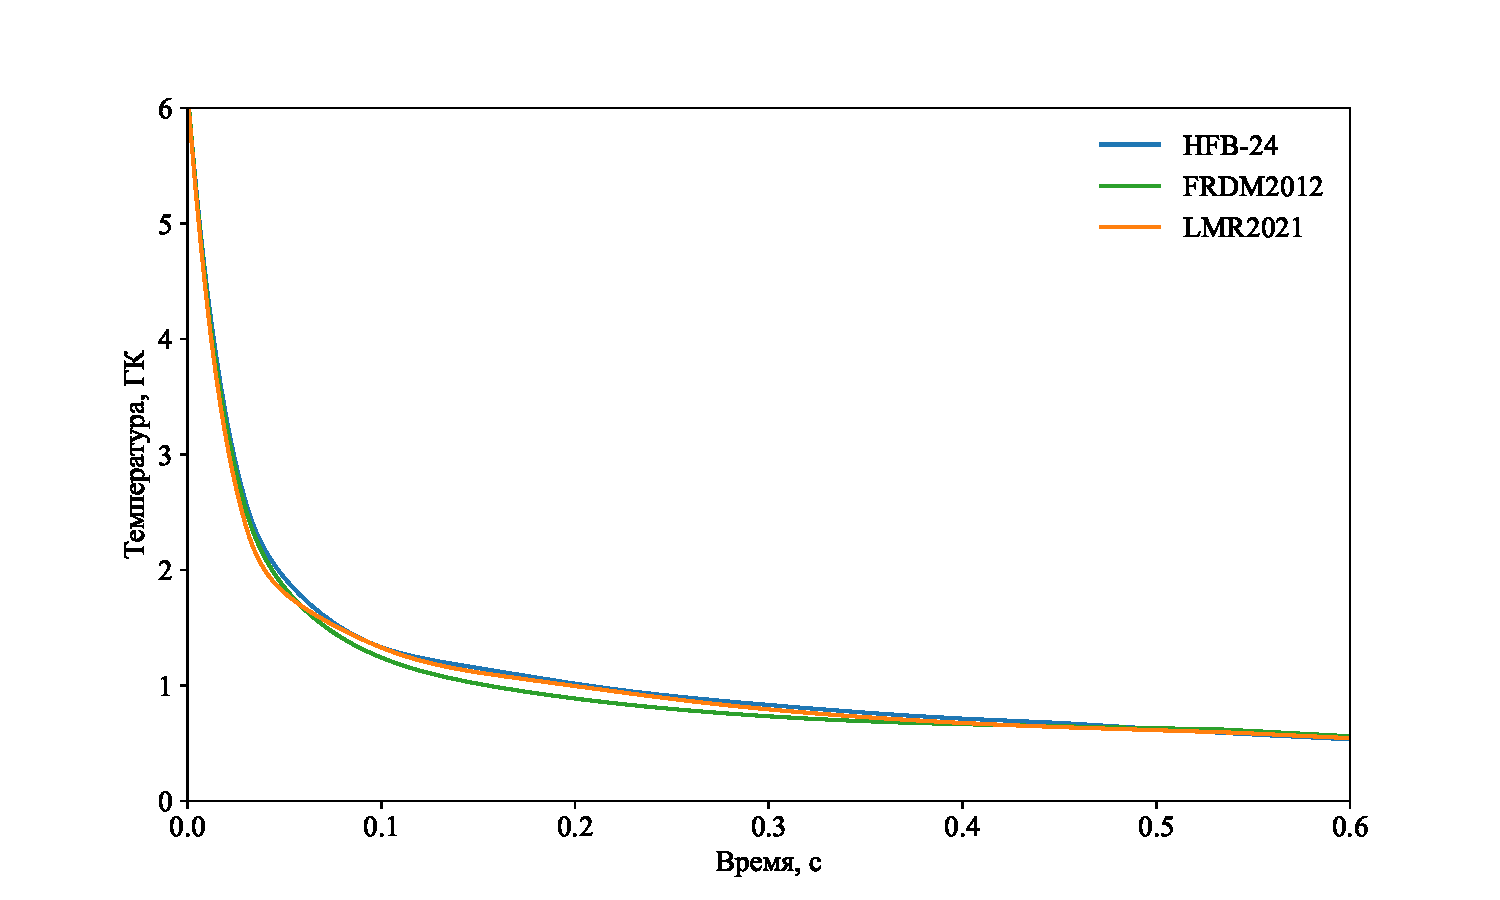
\includegraphics[width=0.9\textwidth]{pics/temp.pdf}
\caption{Изменения температуры системы в первые 600~мс симуляции $r$-процесса в выбросах вещества при слиянии нейтронных звезд. Расчеты проводились с использованием разных моделей ядерных масс.}
\label{fig:temp}
\end{figure}

В случае $r$-процесса основным источником ядерной энергии должны выступать $\beta^-$-распады. Напомним, что библиотеки астрофизических скоростей реакций, которые мы составили в рамках настоящей работы, заимствуют скорости $\beta^-$-распадов из библиотеки REACLIB~\cite{reaclib2010}. Там, где использованная массовая модель выходит за границы REACLIB (практически совпадающие с границами массовой таблицы FRDM2012), скорости недостающих $\beta^-$-распадов вычислялись с помощью экстраполяции.

Полученный результат таким образом ожидаем. Профили температур, полученные в симуляциях с разными массовыми моделями, практически не отличаются, потому что источниками нагрева в расчетах выступал практически один и тот же набор распадов. Тот факт, что на достаточно длительном времени расчета симуляция с моделью FRDM2012 оказываются заметно менее нагретой, чем остальные, объясняется тем, что в двух других библиотеках астрофизических реакций присутствуют дополнительные $\beta^-$-распады сверхнейтроноизбыточных изотопов, до которых волна $r$-процесса доходит как раз в пределах 100~мс. К моменту времени около 400~мс, как видно по рис.~\ref{fig:evolution}, путь $r$-процесса смещается к долине стабильности, и распады этих сверхнейтроноизбыточных изотопов, обеспечивавшие симуляциям с HFB-24 и FRDM2012 добавку ко внутренней энергии, прекращаются, поэтому температуры во всех трех расчетах к концу симуляции сравниваются. 

Хотя разница между профилями температур мала, она все же указывает на важность слабых распадов для моделирования нуклеосинтеза. Если бы составленные нами библиотеки астрофизических скоростей реакций включали также рассчитанные с различными массовыми моделями скорости распадов, влияние масс нейтроноизбыточных изотопов на термодинамику системы могло бы быть более заметным.
